\documentclass[english]{iamthesis}
% changle "slovak" to "english" for english version of the thesis

%----------------------------------------------------------------%
% THESIS DATA

% student name with title e.g. Ing. Martin Klaučo
\def\thesisauthor{Alexey Morozov} 

% year of submmiting to AIS
\def\thesisyear{2020}

% registration number generated by AIS e.g. 19990-50920
\def\thesisnumber{5414-77593} 

% thesis type: BACHELOR|MASTER|DISSERTATION or in slovak 
% BAKALÁRSKA|DIPLOMOVÁ|DIZERTAČNÁ
\def\thesistype{MASTER}

% thesis title
\def\thesistitle{Nonlinear Model Predictive Control of Rotary Pendulum}

% thesis supervisor including degrees e.g. Ing. Martin Klaučo, PhD.
\def\thesissupervisor{Ing. Martin Klaučo, PhD.}

% study field (translate to english if neccesarry) e.g. "Riadenie Procesov" or
% "Process Control"
\def\thesisprogram{Process Control}

% Institute (translate to english if neccesary)
% e.g., "Institute of Information Engineering, Automation, and Mathematics"
\def\thesisinst{Institute of Information Engineering, Automation, and Mathematics}

% Title of the Acknowledgment
% For slovak write: "Poďakovanie" for English write: "Acknowledgment"
\def\thesisack{Acknowledgment}


% End THESIS DATA
%----------------------------------------------------------------%

%----------------------------------------------------------------%
%   Titles and other stuff                                       %
%----------------------------------------------------------------%
\author{\thesisauthor}
\title{\thesistitle}
\date{\today}
\usepackage{layouts}
\usepackage{layout}
%----------------------------------------------------------------%
%   Let the document begin                                       %
%----------------------------------------------------------------%
\begin{document}

% ---------------------------------------------------------------%
% The Frontmatter  !! Do NOT change the structure !!             % 
%----------------------------------------------------------------%

\coverpage

\frontmatter
\pagenumbering{roman}

% include assignment generated by AIS system
%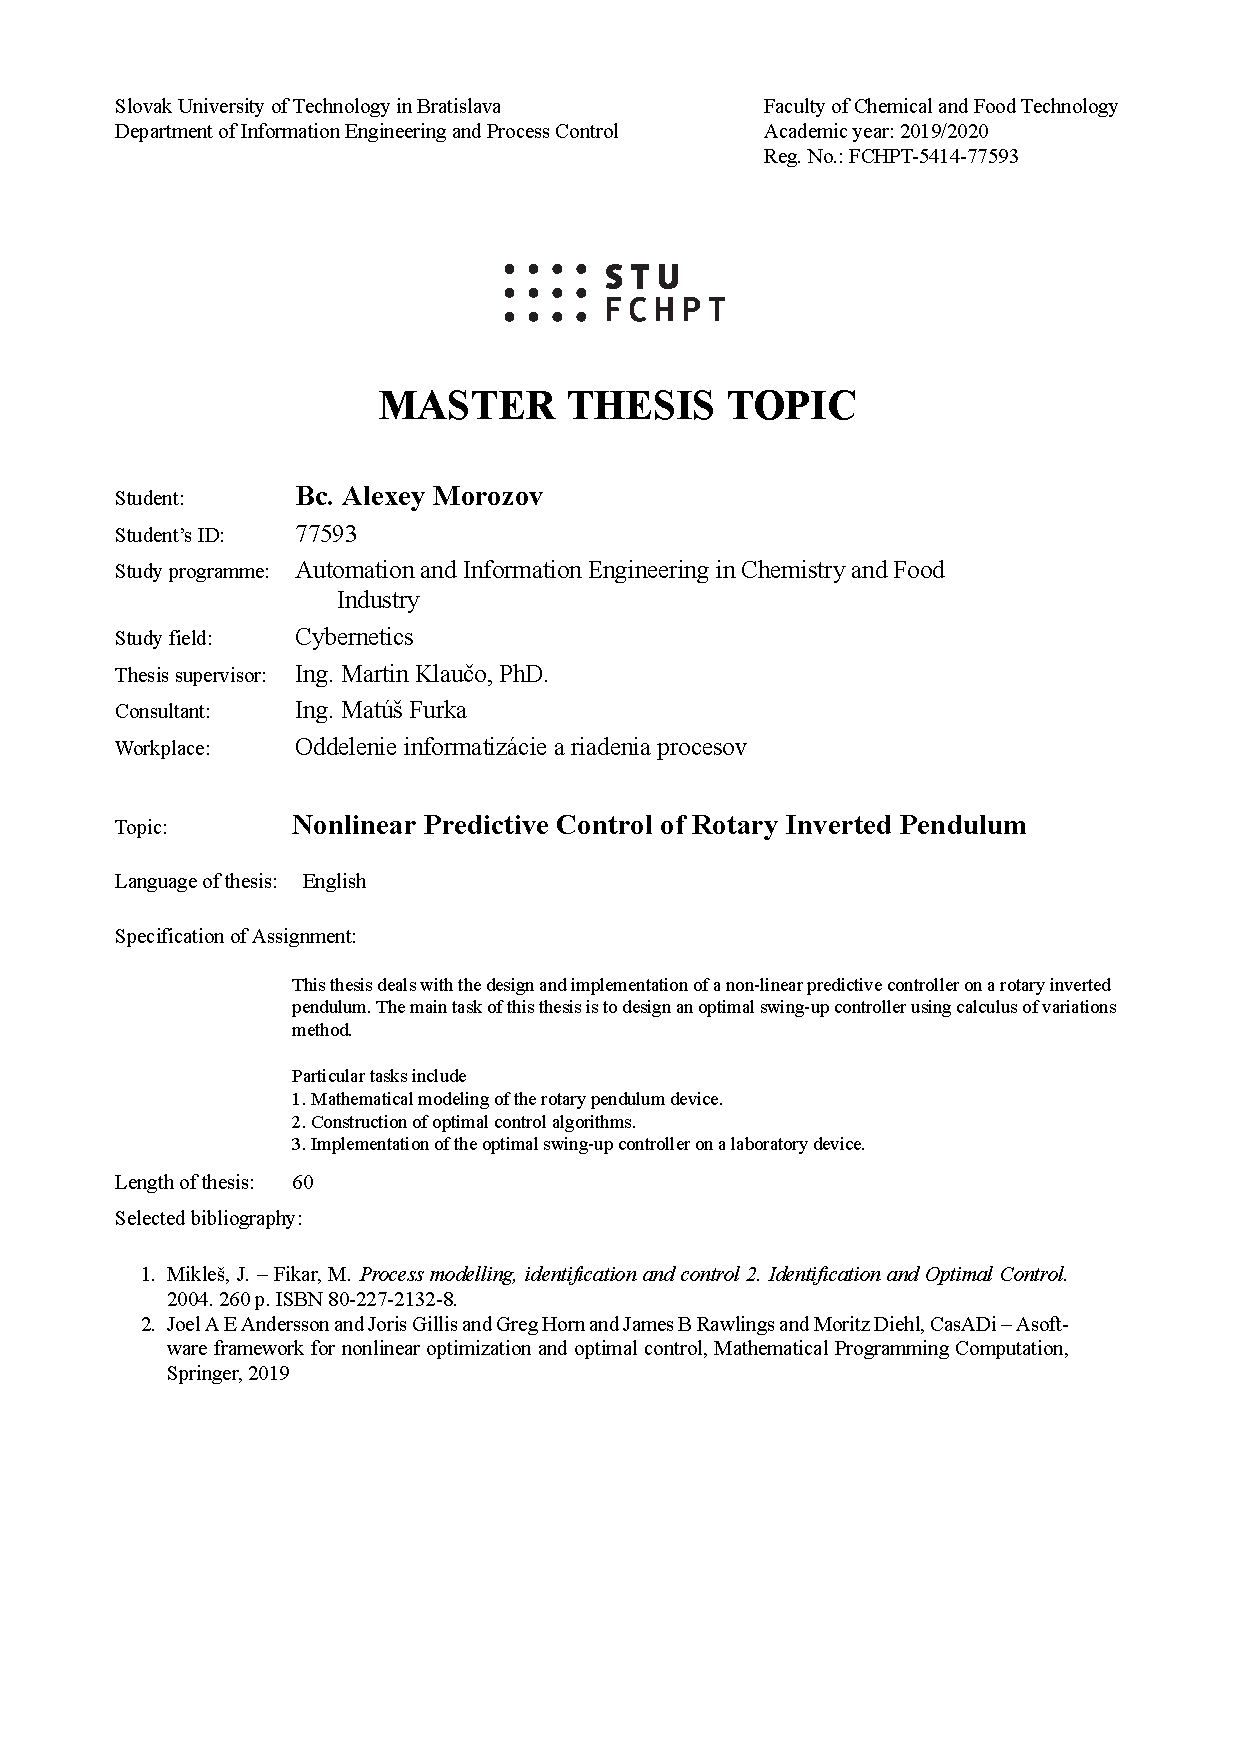
\includepdf[page=1]{content/assignment.pdf}
% use this command only if your assignment has more than 2 pages
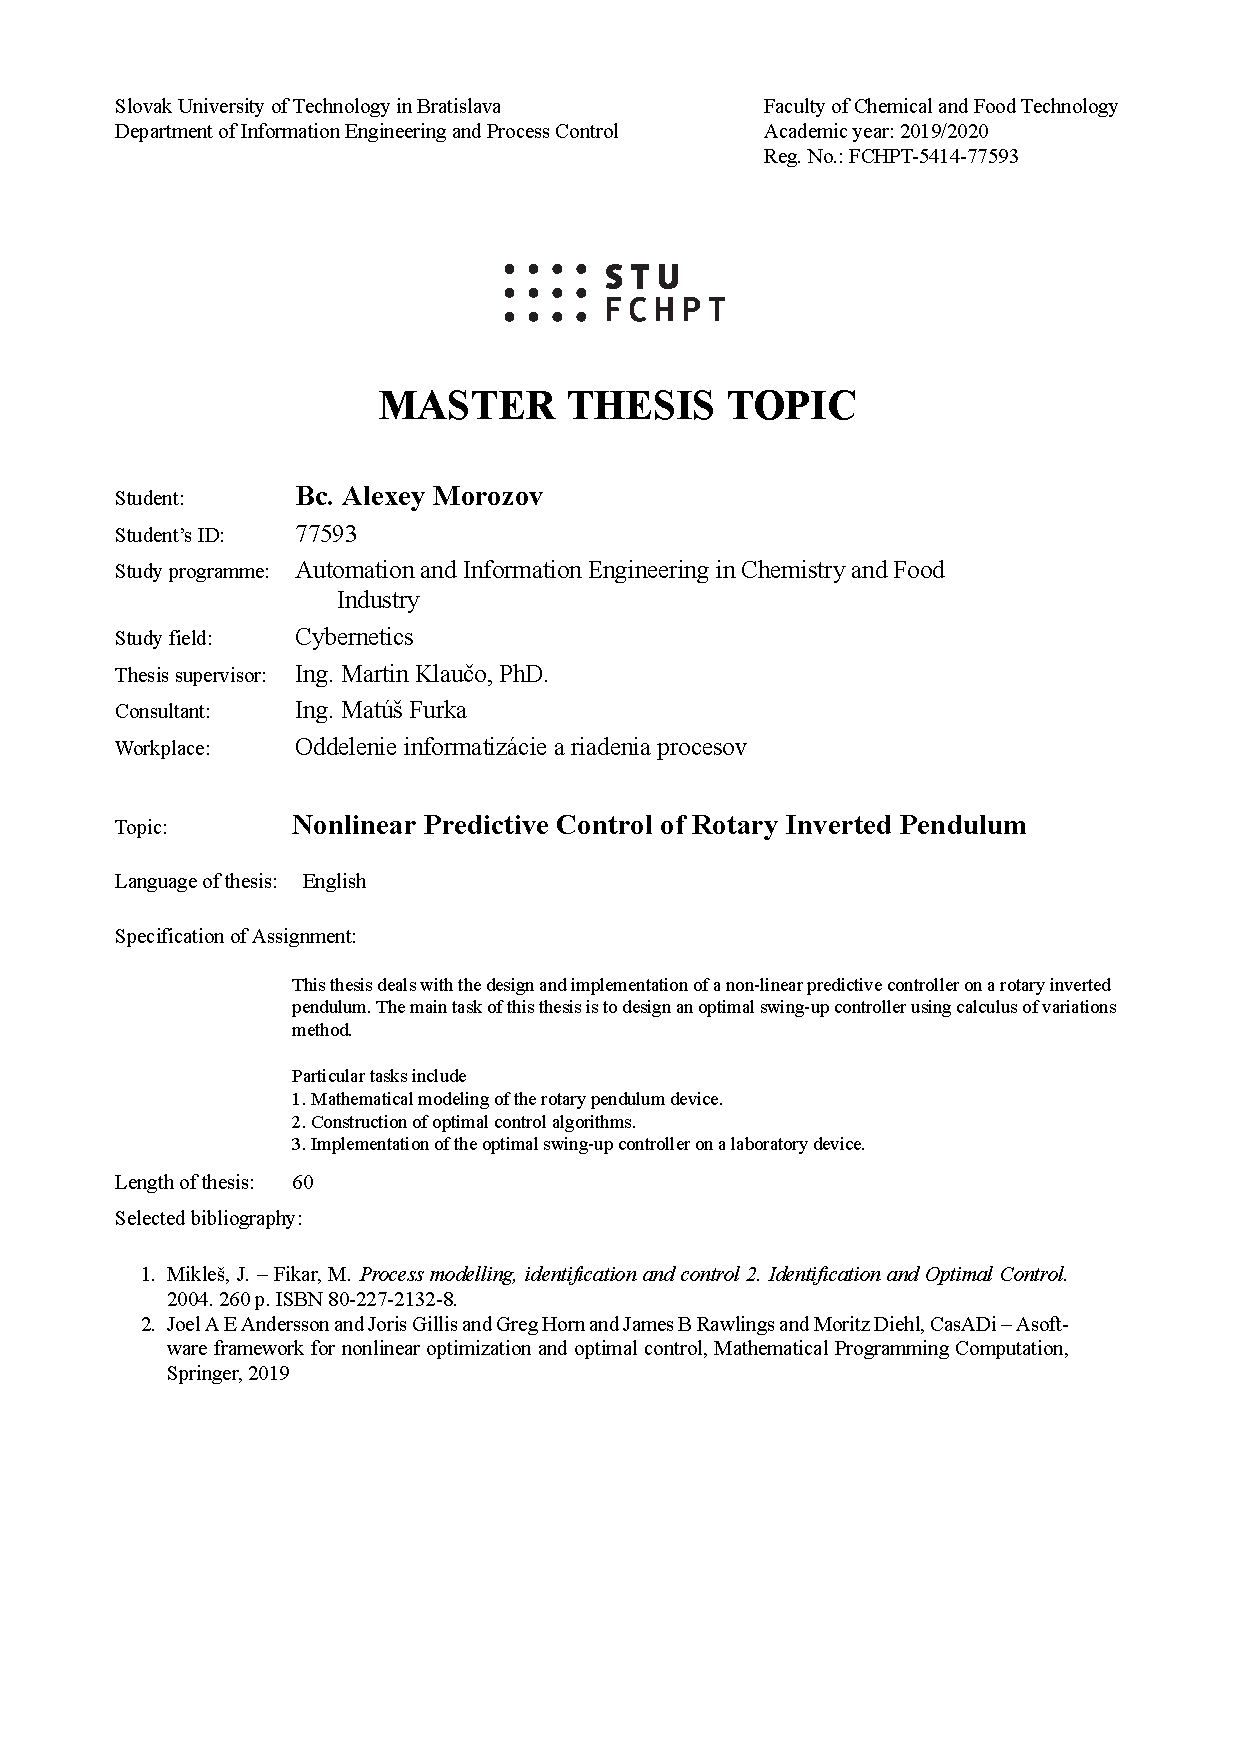
\includepdf[page=2]{content/assignment.pdf}


% do not remove following commands
% do not following commands
\chapter*{\thesisack}
\markboth{}{}
\addcontentsline{toc}{chapter}{\thesisack}
I would like to express my deep gratitude to my supervisor Ing. Martin Klaučo, PhD for his professional guidance, constructive recommendations and useful critiques of this thesis. My grateful thanks are also extended to my consultant Ing. Matúš Furka for his assistance and constructive suggestions during the development of this work. 


\chapter*{Abstract}
\markboth{}{}
\addcontentsline{toc}{chapter}{Abstract}
This work is dedicated to designing control strategies for the rotational inverted pendulum or Furuta’s pendulum. Those strategies are Linear-quadratic regulator (LQR) with the Swing-up controller, Model Predictive Control (MPC) method with the Swing-up controller and the Nonlinear Model Predictive Control (NMPC) strategy. Those controllers are designed in a computing environment MATLAB, for NMPC has used MATMPC toolbox as well as the CasADi toolbox. After verifying in simulations those controllers are used to control the real process.  


\chapter*{Abstrakt}
\markboth{}{}
\addcontentsline{toc}{chapter}{Abstrakt}
Slovenský abstrakt

\setcounter{tocdepth}{2}
\renewcommand{\baselinestretch}{0.1}\normalsize
\tableofcontents
\renewcommand{\baselinestretch}{1.1}\normalsize

% ----------------------------------------------------------------%
% The Mainmatter !! Do NOT change the structure!!                 %
% ----------------------------------------------------------------%
\mainmatter

% individual chapters should be included via a separate tex file, as shown in 
% here. When working in TexStudio (recomennded tool for Win and Mac) set the 
% main.tex as an Explicit root document, so you can compile even you are
% working on other chapter in other tex file.
%
% Open main.tex THEN click Options-> Root Document -> Set Current Document as
% Explicit Root

% introduction
\chapter{Introduction}
\label{ch:intro}
Nowadays Model Predictive Control (MPC) is probably the most advanced control strategy available on the market. This method is based on optimization, so its mathematically provable, that  the calculated control inputs ensure the best control performance for the present scenario, and this is a big advantage. Another, probably even bigger advantage of MPC, is that different physical limitations of the process and constrains on measured variables, control variables, and controlled variables are the part of that optimization problem. And if that optimization problem is feasible, we can guarantee, that those constraints would not be violated during the plant operation. As it is a predictive control strategy, it uses accurate model predictions of the future behavior of the system and can provide early warnings of potential problems.

As we can see an MPC is a great control strategy. But nothing in this world is for free and MPC is not an exception. The MPC strategy is expensive, both in time and resources. MPC solves an optimization problem. This optimization problem could also be both equality and inequality constrained. And the presence of these constraints can make the optimization problem extremely difficult to solve. Therefore pretty strong computation machines are required. The MPC also requires an appropriate process model to compute accurate predictions. And the main industrial restriction on MPC is time. Most of the industrial problems are really complicated because of the high number of process and manipulated variables and their intercations. And the MPC must be able to solve such problems during only one sampling period.

This thesis is dedicated to designing a predictive controller, that deals with the main restrictions on MPC such as short available time to solve an optimization problem and nonlinear constraints. To test such MPC the Furuta Pendulum is used. Furuta pendulum is a rotational inverted pendulum and it is a great example of a fast, nonlinear process with complex dynamics. It was invented in 1992 at the Tokyo Institute of Technology by Katsuhisa as an example of a complex nonlinear oscillator, on the purpose of process control algorithm testing. This pendulum is underactuated and extremely non-linear due to gravitational forces and Coriolis interactions. As the main task of the thesis is to perform a swing-up control of the pendulum, two different approaches are used: first is a heuristic swing-up control, where the pendulum is controlled by two controllers: energy-shaping controller and a linear MPC. The second approach is an optimal swing-up control, where a Nonlinear Model Predictive Control (NMPC) strategy is used.

The thesis consists of two main parts: the first is a theoretical foundation, and the second illustrates simulation control of the pendulum device. In the first part operation of the pendulum is explained and its mathematical model derived. Also in that part, the theory for individual controllers is described. In the second part, both heuristic and optimal swing-up control approaches are explained as well as \textsc{MATLAB} implementation, and the results of the control are illustrated.   

% theory
\chapter{Theory}

\section{Furuta's Pendulum}

Rotational inverted pendulum or Furuta’s pendulum composes of two main parts: motor-driven arm, which rotates in the horizontal plane and a pendulum, attached to that arm, which freely rotates in the vertical plane. The system is underactuated and extremely nonlinear due to the gravitational forces and the coupling arising from the Coriolis and centripetal forces. The schematic representation of the pendulum is shown in \ref{furuta}
\begin{figure}[h]
	\centering
	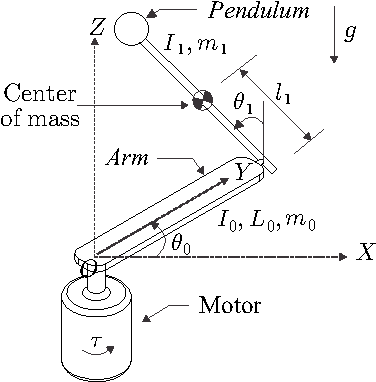
\includegraphics[width=.6\linewidth]{images/furuta}
	\caption{Furuta's Pendulum}
	\label{furuta}
\end{figure}
\newpage
The symbols in the figure indicate the following:
\begin{itemize}
	\item \textbf{$g$} - gravitational acceleration [\si{\metre\per\square\second}]
	\item \textbf{$m_0$} - mass of arm [\si{\kilogram}]
	\item \textbf{$m_1$} - mass of pendulum [\si{\kilogram}]
	\item \textbf{$L_0$} - length of arm [\si{\metre}]
	\item \textbf{$L_1$} - length of pendulum [\si{\metre}]
	\item \textbf{$l_1$} - location of the pendulums center of mass [\si{\metre}]
	\item \textbf{$I_0$} - moment of inertia of arm [\si{\kilogram\per\square\metre}]
	\item \textbf{$I_1$} - moment of inertia of pendulum [\si{\kilogram\per\square\metre}]
	\item \textbf{$\theta_0$} - arm angle [\si{\radian}]
	\item \textbf{$\theta_1$} - pendulum angle [\si{\radian}]
	\item \textbf{$\tau$} - motor torque [\si{\volt}]
\end{itemize}
\subsection{State-Space Representation}
To obtain the state representation of the process we must define our state variables first:
\begin{equation}
	\begin{bmatrix}
	x_1 & x_2 & x_3 & x_4
	\end{bmatrix}^\intercal = 
	\begin{bmatrix}
	\theta_0 & \dot{\theta_0} & \theta_1 & \dot{\theta_1}
	\end{bmatrix}^\intercal
\end{equation}
Control variable:
\begin{equation} u = \tau \end{equation}
Then we can write our state equations:
\begin{subequations}
\begin{equation}\dot{x_1} = \dot{\theta_0} \end{equation}
\begin{equation}\dot{x_2} = \frac{\gamma(\epsilon\dot{\theta_0}^2+\rho)-\delta(\tau+\beta\dot{\theta_1}^2-\sigma\dot{\theta_0}\dot{\theta_1})}{\gamma^2-\alpha\delta}\end{equation}
\begin{equation}\dot{x_3} = \dot{\theta_1}\end{equation}
\begin{equation}\dot{x_4} = \frac{\gamma(\tau+\beta\dot{\theta_1}^2-\sigma\dot{\theta_0}\dot{\theta_1})-\alpha(\epsilon\dot{\theta_0}^2+\rho)}{\gamma^2-\alpha\delta}\end{equation}
\end{subequations}
where
\begin{equation}\alpha = I_0+L_0^2m_1+l_1^2m_1\sin^2\theta_1\end{equation}
\begin{equation}\beta = L_0m_1l_1\sin\theta_1 \end{equation}
\begin{equation}\gamma = L_0m_1l_1\cos\theta_1\end{equation}
\begin{equation}\delta = I_1+l_1^2m_1\end{equation}
\begin{equation}\epsilon = l^2_1m_1\sin\theta_1\cos\theta_1\end{equation}
\begin{equation}\rho = m_1gl_1\sin\theta_1\end{equation}
\begin{equation}\tau = 2l^2_1m_1\sin\theta_1\cos\theta_1\end{equation}
Now these non-linear differential equations we can write in the form of matrices:
\begin{equation}\label{nonlinmodel}
\begin{bmatrix}
\dot{x_1} \\ \dot{x_2} \\ \dot{x_3} \\ \dot{x_4}
\end{bmatrix} = \begin{bmatrix}
\dot{\theta_0}\\
\frac{\gamma(\epsilon\dot{\theta_0}^2+\rho)-\delta(\tau+\beta\dot{\theta_1}^2-\sigma\dot{\theta_0}\dot{\theta_1})}{\gamma^2-\alpha\delta}\\
\dot{\theta_1}\\
 \frac{\gamma(\tau+\beta\dot{\theta_1}^2-\sigma\dot{\theta_0}\dot{\theta_1})-\alpha(\epsilon\dot{\theta_0}^2+\rho)}{\gamma^2-\alpha\delta}
\end{bmatrix}
\end{equation}
or:
\begin{equation}\dot{x} = f(x,u) =\begin{bmatrix}f_1(x,u)\\f_2(x,u)\\f_3(x,u)\\f_4(x,u)\end{bmatrix} \end{equation}
So that’s our non-linear dynamic model of the process. But only the NMPC controller is able to operate with such a model.  So, to make that model suitable for LQR and MPC controller we can approximate that non-linear model by a linear model as follows:
\begin{equation}\dot{x} = Ax + Bu\end{equation}
And the constant matrices are derived as:
\begin{equation}
A = \begin{bmatrix}
\frac{\partial f_1(x,u)}{\partial x_1}&\frac{\partial f_1(x,u)}{\partial x_2}&\frac{\partial f_1(x,u)}{\partial x_3}&\frac{\partial f_1(x,u)}{\partial x_4}\\
\frac{\partial f_2(x,u)}{\partial x_1}&\frac{\partial f_2(x,u)}{\partial x_2}&\frac{\partial f_2(x,u)}{\partial x_3}&\frac{\partial f_2(x,u)}{\partial x_4}\\
\frac{\partial f_3(x,u)}{\partial x_1}&\frac{\partial f_3(x,u)}{\partial x_2}&\frac{\partial f_3(x,u)}{\partial x_3}&\frac{\partial f_3(x,u)}{\partial x_4}\\
\frac{\partial f_4(x,u)}{\partial x_1}&\frac{\partial f_4(x,u)}{\partial x_2}&\frac{\partial f_4(x,u)}{\partial x_3}&\frac{\partial f_4(x,u)}{\partial x_4}
\end{bmatrix}
\end{equation}
respektive:
\begin{equation}
	A =\begin{bmatrix}0&1&0&0\\
	0&0&\frac{-gL_0l_1^2m_1^2}{(m_1L_0^2+I_0)(m_1l_1^2+I_1)-L_0^2l_1^2m_1^2}&0\\
	0&0&0&1\\
	0&0&\frac{gl_1m_1(m_1L_0^2+I_0)}{(m_1L_0^2+I_0)(m_1l_1^2+I_1)-L_0^2l_1^2m_1^2}&0
	\end{bmatrix}
\end{equation}
\begin{equation}B = \begin{bmatrix}
\frac{\partial f_1(x,u)}{\partial u}\\\frac{\partial f_2(x,u)}{\partial u}\\\frac{\partial f_3(x,u)}{\partial u}\\\frac{\partial f_4(x,u)}{\partial u}
\end{bmatrix}=\begin{bmatrix}
0\\ 
\frac{m_1L_1^2+I_1}{(m_1L_0^2+I_0)(m_1l_1^2+I_1)-L_0^2l_1^2m_1^2}\\0\\
\frac{-L_0l_1m_1}{(m_1L_0^2+I_0)(m_1l_1^2+I_1)-L_0^2l_1^2m_1^2}
\end{bmatrix}\end{equation}
\begin{equation}C = \begin{bmatrix}0&0&1&0\end{bmatrix}\end{equation}
\begin{equation}D = 0\end{equation}
The linearized equations of motion for the simplified system are now could be derived for two equilibrium positions: upright and downward. The reason is that at the downward position the system's output, which is the position of the pendulum, has a stable point at “$+\pi$” and “$-\pi$”, while at the upright position system has no stable point.\\

The model, obtained by linearization around the upright operation point, is used for fulfilling the main control objective, which is stabilizing the pendulum at the upright position. The second model is used to simulate process behavior during initial excitation by a Swing-up controller.
\section{Controller Synthesis}
\subsection{LQR design}
The Linear Quadratic Regulator (LQR) is a well-known method that provides optimally controlled feedback gains to enable the closed-loop stable and high performance design of systems.
\begin{equation}
\begin{split}
\dot{x} &= Ax + Bu\\
y &= Cx, C=I^{n \times n}
\end{split}
\end{equation}
which requires  full-state feedback (all n states are measurable).
The feedback gain is a matrix K and the feedback control law takes the form:
\begin{equation}
	u = -Kx
\end{equation}
Than closed-loop system dynamics can be written:
\begin{equation}
\dot{x} = (A-BK)x
\end{equation}
So there appears condition that poles of $(A-BK)$ must be in in stable, suitably-damped locations in the complex plane.
\subsubsection{Derivation of LQR}
Towards a generic procedure for solving optimal control problems, we derive a methodology based on the calculus of variations. The problem statement for a fixed final time $t_f$ is:
\begin{equation}
\begin{split}
	J = \min_{u}& \quad \Phi(t_f)+\frac{1}{2}\int\limits_{t_0}^{t_f}L(x(t),u(t),t)\;dt\\
	s.t.&\quad  \dot{x} = f(x(t),u(t),t)\\
	& \quad x(t_0) = x_0
	\end{split}
\end{equation}
In the case of the Linear Quadratic Regulator (with zero terminal cost), we set  $\Phi(x(t_f))=0$, and $L = x^\intercal Qx+u^\intercal Ru$ solve the new optimization problem
\begin{equation}
J=\min_{u}  \frac{1}{2}\int\limits_{t_0}^{t_f}x^\intercal Qx+u^\intercal Ru\;dt
\end{equation}
Where $Q$ and $R$ are positive semidefinite weighting matrices for states and control input respectively.
Now we define new variable $H$ as:
\begin{equation}
H = \frac{1}{2}(x\intercal Qx + u^\intercal Ru)+\lambda^\intercal(Ax + Bu)
\end{equation}

As we are looking for minimum, we apply the condition, that $\frac{\partial H(x,u,\lambda)}{\partial u}$ is equal to zero.
\begin{equation}
	\frac{\partial H(x,u,\lambda)}{\partial u} = Ru + B^\intercal\lambda = 0
\end{equation}
then:
\begin{equation}
u = -R^{-1}B^\intercal\lambda
\end{equation}
where
\begin{equation}
\lambda = Px
\end{equation}
and finally
\begin{equation}
u = -R^{-1}B^\intercal Px
\end{equation}
And that is our optimal control law for full-state feedback LQR. Matrix $P$ is calculated by solving Riccati equation in continuous time:
\begin{equation}
Q + A^\intercal P + PA - PBR^{-1}B^\intercal P = 0
\end{equation}
\subsection{MPC controller design}
MPC uses a model of the system to make predictions about the system’s future behavior. MPC solves an online optimization algorithm to find the optimal control action that drives the predicted output to the reference. MPC can handle MIMO systems that may have interactions between their inputs and outputs. It can also handle input and output constraints. MPC has preview capability; it can incorporate future reference information into the control problem to improve controller performance.
\subsubsection{MPC formulation}
MPC controller requires the model of the system in the discrete time formulation that
is used to predict systems behavior in the future:
\begin{equation}
	\begin{split}
	&x_{k+1} = Ax_k + Bu_k\\
	&y_k = Cx_k
	\end{split}
\end{equation}
State predictions: 
\begin{equation}
\begin{split}
\hat{x}_{k+1} &= Ax_k + Bu_k\\
\hat{x}_{k+2} &= A\hat{x}_{k+1} + Bu_{k+1}\\
&= A^2x_k + ABu_k + Bu_{k+1}\\
\hat{x}_{k+3} &= A\hat{x}_{k+2} + Bu_{k+2}\\
&= A^3x_k + A^2Bu_k + ABu_{k+1} + Bu_{k+2}\\
&\vdots\\
\hat{x}_{k+N} &= A^Nx_k+\sum_{j=k}^{k+N-1}A^jBu_{k+N-j-1}
\end{split}
\end{equation}
Output Predictions:
\begin{equation}
\begin{split}
\hat{y}_{k+1} &= C\hat{x}_{k+1}\\
			  &= CAx_k + CBu_k\\
\hat{y}_{k+2} &= C\hat{x}_{k+2}\\
			  &= CA^2x_k + CABu_k + CBu_{k+1}\\
			  \hat{y}_{k+2} &= C\hat{x}_{k+2}\\
			  &= CA^3x_k + CA^2Bu_k + CABu_{k+1} + CBu_{k+2}
\end{split}
\end{equation}
Now we can obtain predictive system model:
\begin{equation}
	\begin{bmatrix}
	\hat{y}_{k+1}\\\hat{y}_{k+2}\\ \vdots\\ \hat{y}_{k+N}
	\end{bmatrix} = \begin{bmatrix}CA\\CA^2\\ \vdots \\ CA^N\end{bmatrix}x_k + \begin{bmatrix}CB& 0&\cdots&0\\
	CAB&CB&\cdots&0\\
	\vdots&\vdots&\ddots&\vdots\\
	CA^{N-1}&CA^{N-2}&\cdots&CB\end{bmatrix}\begin{bmatrix}u_k\\u_{k+1}\\\vdots\\u_{k+N-1}\end{bmatrix}
\end{equation}
respektive:
\begin{equation}
	\hat{Y} = Y_0 + GU
\end{equation}
And now the whole optimization problem could be written as a QP problem with constrains:
\begin{equation}\label{mpcformulation}
\begin{split}
J = \min_{u}& \sum_{k}^{k+N}x^\intercal Q_xx+u^\intercal Q_uu\\
s.t.&\quad  x_{k+1} = Ax_k + Bu_k\\
&\quad  y_{k} = Cx_k\\
& \quad u_{min}\leq u_k\leq u_{max}
\end{split}
\end{equation}
Where $Q_x$ and $Q_u$ are positive semidefinite weighting matrices for states and control input respectively.
By solving that optimization problem we get the optimal value for control input for every simulation step.
\subsection{Swing-Up controller design}
For initial excitation of the system we use the energy-based swing-up controller. The strategy with this controller is that we increase the amplitude of swings by increasing the energy of the system with every swing. The energy is added by controlling arms movements and depends on the actual energy of the pendulum. The actual energy of the pendulum can be calculated from the actual position of the pendulum and its velocity: 
\begin{equation}
E = \frac{m_1gl_1}{2}((\frac{\dot{\theta_1}}{\omega_0})^2+\cos\theta_1 - 1)
\end{equation}
Than the control law has following form:
\begin{equation}
	u = k_vEsign(\dot{\theta_1}\cos\theta_1)
\end{equation}
Where element $sign(\dot{\theta_1}\cos\theta_1)$ determines direction i which the force will be applied and $k_vE$ is the gain of the controller.









\chapter{Case Study}
In this section the theory from Section \ref{mpcsection}, Sections \ref{energyshapingsection} and Sections \ref{nmpcsection} in attempt design and tested in simulations an optimal controllers, suitable to control the real device Fig.\ref{furutareal}
\begin{figure}[H]
	\centering
	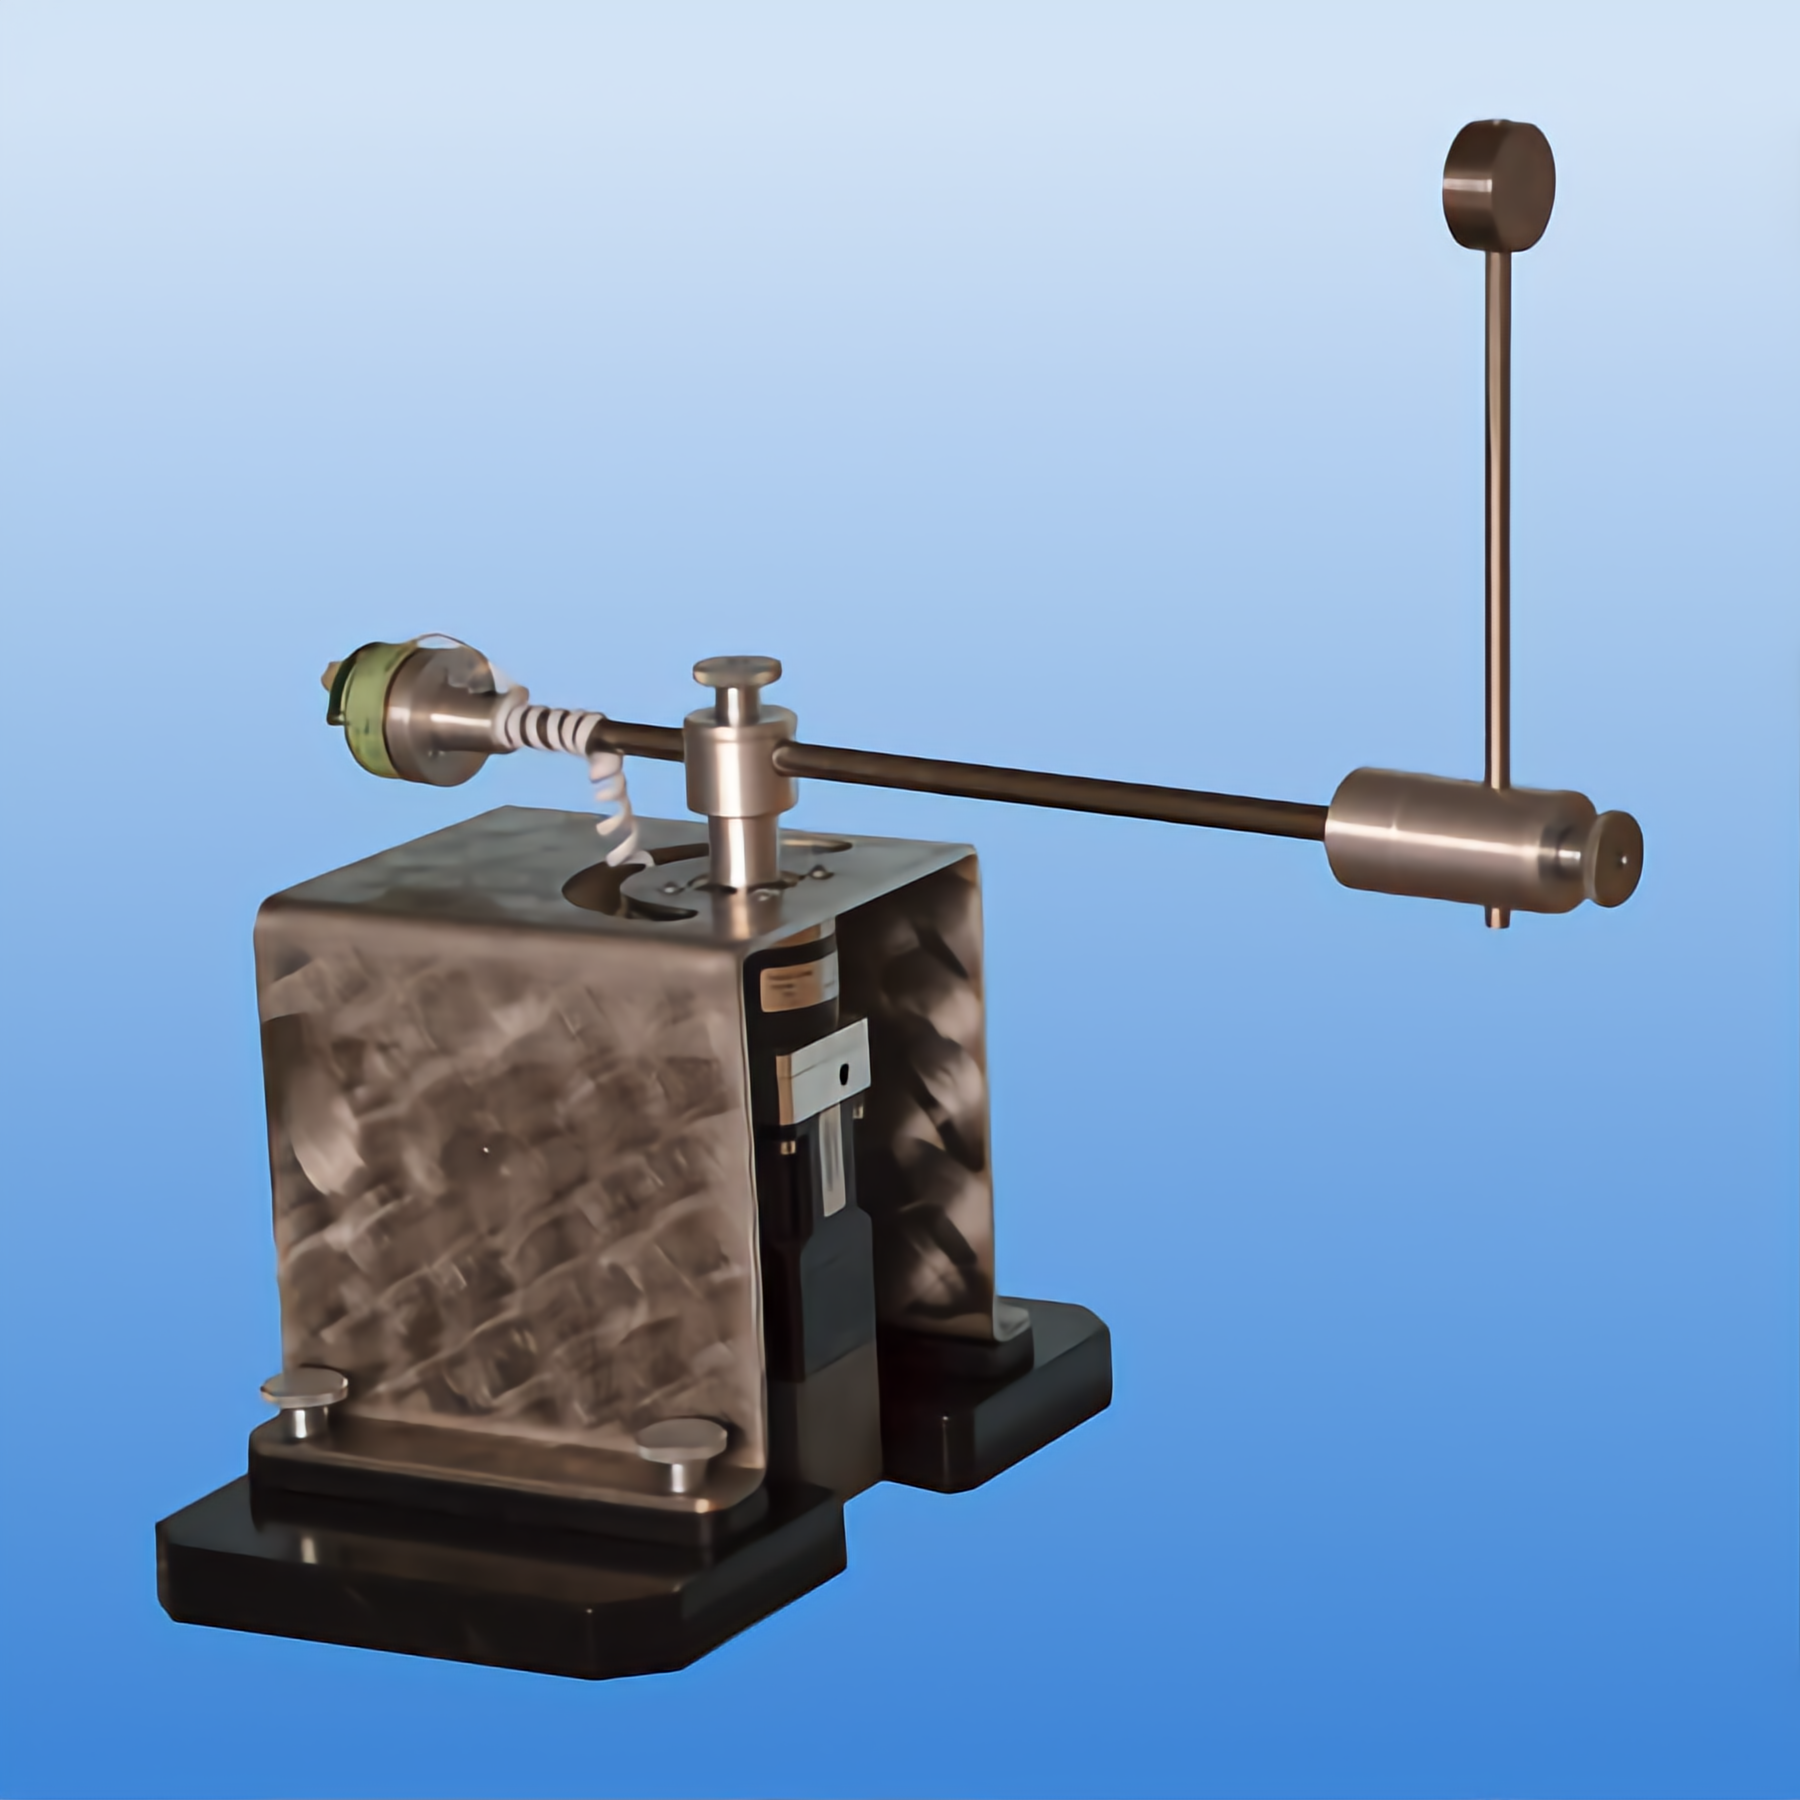
\includegraphics[width=.6\linewidth]{images/furutareal}
	\caption{Laboratory Furuta pendulum device}
	\label{furutareal}
\end{figure}
which values of parametres are given in the following table
\begin{table}[H]
	\caption{Values of Furuta Pendulum Parameters}

\begin{tabular}{l l l}	
	\noalign{\hrule height 1pt}
	Parameter&Symbol&Value\\
	\noalign{\hrule height 1pt}
	Gravitational acceleration&$g$&9.81\si{\metre\per\square\second}\\
	Mass of arm&$m_0$&0.6 \si{\kilogram}\\
	Mass of pendulum&$m_1$&0.198 \si{\kilogram}\\
	Length of arm&$L_0$&0.51 \si{\metre}\\
	Llength of pendulum&$L_1$&0.23 \si{\metre}\\
	Location of the pendulums center of mass&$l_1$&0.21 \si{\metre}\\
	Moment of inertia of arm&$I_0$&0.052 \si{\kilogram\per\square\metre}\\
	Moment of inertia of pendulum&$I_1$&8.72e-4 \si{\kilogram\per\square\metre}\\
	Sampling time&$T_s$&0.02 \si{\second}\\
	\hline
\end{tabular}
\label{furuta:values}
\end{table}
By substituting values from table \ref{furuta:values} into \ref{linSSmodel:general} and evaluating it at the upright operation point 
\begin{equation}
\ui{x}{up} = \begin{bmatrix}0,0,0,0\end{bmatrix}^\intercal, 
\end{equation}
the linear, continuouss-time State-Space model, representing the dynamic of the pendulum near the upright position is obtained
\begin{subequations}\label{linSSmodel:up}
	\begin{align}
	\ui{A}{c,up} &=\begin{bmatrix}
	0&1&\ 0& 0\\
	0&0&-15.8833&0\\
	0&0&\ 0&1\\
	0&0&\ \; \,77.5373&0
	\end{bmatrix},\\
	\ui{B}{c,up} &=\begin{bmatrix}
	\ 0\\
	\ \; \,17.6366\\
	\ 0\\
	-38.9393
	\end{bmatrix}.
	\end{align}
\end{subequations}
And with this model obtained, we are ready to proceed to controller design and pendulum control.
 
First a linear MPC strategy to stabilize the pendulum at the upright pozition will be designed. Second is the Energy-Shaping controller to swing the pendulum from the downside position. Then the MPC and Swing-Up controllers will be combined to perform Heuristic Swing-Up control of the pendulum. And finally via using a NMPC strategy an Optimal Swing-Up control of the pendulum will be performed.
\section{Model Predictive Controller}
Due to the pendulums setup, the MPC formulation (\ref{mpcgeneral}) could be applied directly. As known, a linear MPC uses a linear prediction model \ref{linSSmodel:up} of the process to predict the behavior of the system over the prediction horizon. Such a predictive model is only relevant in vicinity of linearization point. That is the reason why the linear MPC strategy is used to conrol the pendulum only around upright position. 
The MPC is a discrete-time strategy, therefore the first step of the construction of such a controller is to obtain the discrete-time linear predictive model. Such model can be derived from continuous-time model (\ref{linSSmodel:up}) by some discretization method. In this thesis a zero-order hold method, with the discretization step, equal to devices sampling time, $0.02 s$ is used. 
\begin{subequations}\label{dismatrices}
	\begin{align}
	\ui{A}{d} &=\begin{bmatrix}
	1&0.02&-0.0032& 0\\
	0&1&-0.3193&-0.0032\\
	0&0&\ \; \,1.0155&\ \; \,0.0201\\
	0&0&\ \; \,1.5588&\ \; \,1.0155
	\end{bmatrix},\\
	\ui{B}{d} &=\begin{bmatrix}
	\ \; \,0.0035\\
	\ \; \,0.3536\\
	-0.0078\\
	-0.7828
	\end{bmatrix}.\\
	\end{align}
\end{subequations}
The output matrices remain unchanged from (\ref{linmatrices}).\\ 

Now it is important to determine the range around the linearization point, where such a model is relevant. For that purpose will be evaluated the difference in outputs from the non-linear and linear model. For that purpose both models will be simulated with the same value of control input.
\begin{table}[H]
	\caption{Comparisson of linear and non-linear models}
	\label{models:comparisson}
\begin{tabular}{c c}	
	\noalign{\hrule height 1pt}
	Initial angle of the pendulum [deg]&Difference in outputs [deg]\\
	\noalign{\hrule height 1pt}
	30&0.5977\\
	40&0.8370\\
	50&1.0200\\
	60&1.1474\\
	70&1.2314\\
	\hline
\end{tabular}
\end{table}
Those results demonstrate that an MPC can be used to control the pendulum roughly in $\pm50deg$ around the upright position. Also, those results were obtained for the limit value of control input, for a smaller value of control input the difference, naturally, will be lesser.\\

The next, probably the most important, step is to design weight matrices $\ui{Q}{x}$ and $\ui{Q}{u}$. The main weights must be given to the position of the pendulum, what is our main controlled parameter, and the position of the arm, to prevent the possible scenario when the pendulum is stabilized at the upright position and the arm rotates constantly. 
\begin{equation}
\ui{Q}{x} = \begin{bmatrix}
1.5&0&0&0\\
0&0.08&0&0\\
0&0&10&0\\
0&0&0&0.2
\end{bmatrix}, \quad \ui{Q}{u} = 1.
\end{equation}
Weight matrices are the key point of MPC, as through them we define for MPC a requested control performance.
The remain MPC parametres can be set as shown in the following table
\begin{table}[H]
	\caption{MPC parameters during the stabilization at the upright position}
	\begin{tabular}{l c c}
		\noalign{\hrule height 1pt}
		Parameter&Symbol&Value\\
		\noalign{\hrule height 1pt}
		Prediction horizon&$N$&$20$\\
		Initial condition&$x_0$&$\begin{bmatrix}-1,-2,0.5,2\end{bmatrix}^\intercal$\\
		Constraint on control input-upper bound&$\ui{u}{max}$&$\ \; \,10$\\
		Constraint on control input-lower bound&$\ui{u}{min}$&$-10$\\
		\hline
	\end{tabular}
\end{table}
Due to the fact, that the Furuta pendulum performs a rotary motion, the safety constraints on the states are not necessary. So only present inequality constraints are the limit constraints on the control input.\\

Considering all aforesaid, the MPC formulation can be written in the following form
\begin{subequations}\label{mpc:linear}
	\begin{align}
	\min_{U}\ &\sum_{k=0}^{N-1} \lrp{\left\| \ui{Q}{x}x_{k}\right\|_2+\left\|\ui{Q}{u}u_{k}\right\|_2}\\
	\text{s.t.}\ &x_{k+1} = A_dx_{k} + B_du_{k}\qquad\qquad\ \ \,  k \in \mathbb{N}_0^{N-1}\\
	&x_0 = x(0)\\
	&\ui{u}{min}\leq u_{k}\leq \ui{u}{max}\qquad\qquad\qquad\;   k \in \mathbb{N}_0^{N-1}
	\end{align}
\end{subequations}
This predictive controller is designed in \textsc{MATLAB}, using the \textsc{YALMIP} toolbox \cite{YALMIP} to formulate the problem and \textsc{Gurobi} solver to solve it.
\newpage
\begin{figure}[H]
	\centering
	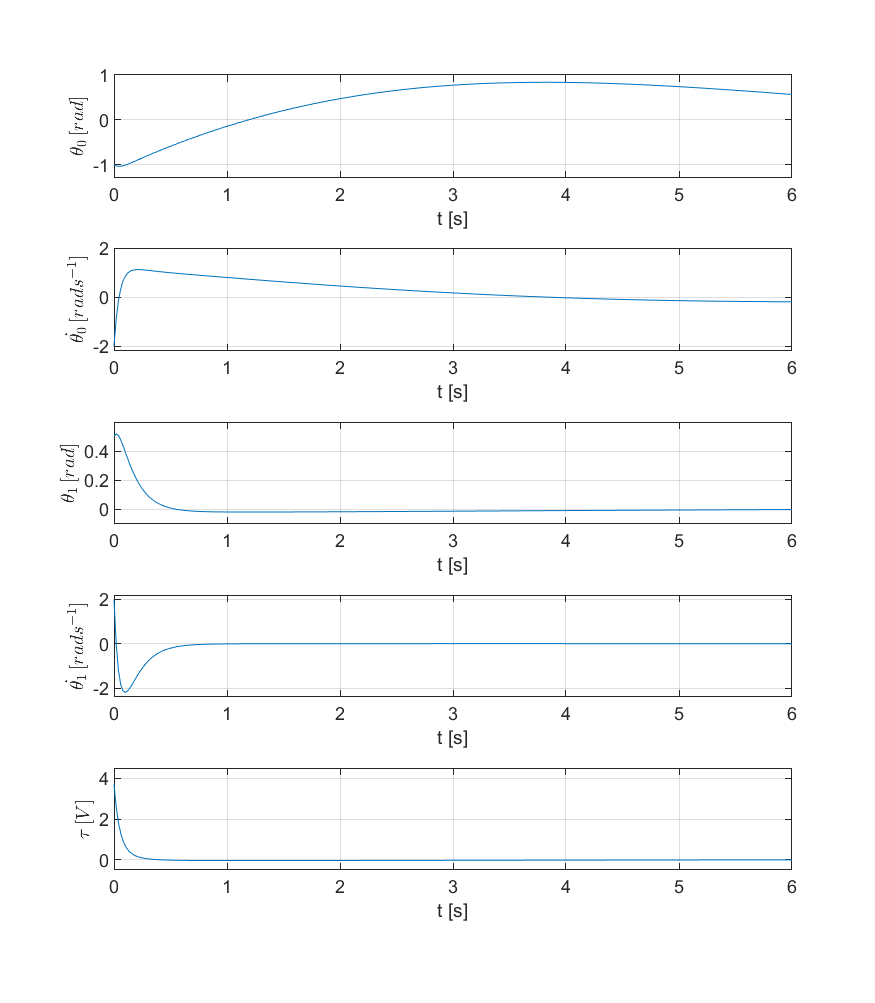
\includegraphics[width=1.1\linewidth]{images/MPC}
	\caption{Simulation results for a scenario with stabilization at the upright position by linear MPC. The plots depict, respectively, the individual states , the third of which is the controlled pendulum position $\theta_1(t)$, and the control input $\tau(t)$.}
	\label{mpc}
\end{figure}
The simulation results of stabilizing the pendulum at the upright position, using a linear MPC are shown in Fig.\ref{mpc}. As can be observed, such a predictive controller is capable of stabilizing the pendulum, without constraints violation. The only issue is the solving time. For this scenario, the solving time was $[0.0156, 0.0313]s$, which is not satisfying because of sample time. One possible solution is the hardware upgrade, as the simulations were performed on a rather old laptop.

\section{Energy-Shaping Controller}
The main purpose of the Energy-Shaping controller is to swing the pendulum from the downside position into the upright position where the control of the process will be taken by another controller. 
Such controller can be designed by applying the control law (\ref{energy-shaping}) directly as a state-feedback controller.
\newpage
\begin{figure}[H]
	\centering
	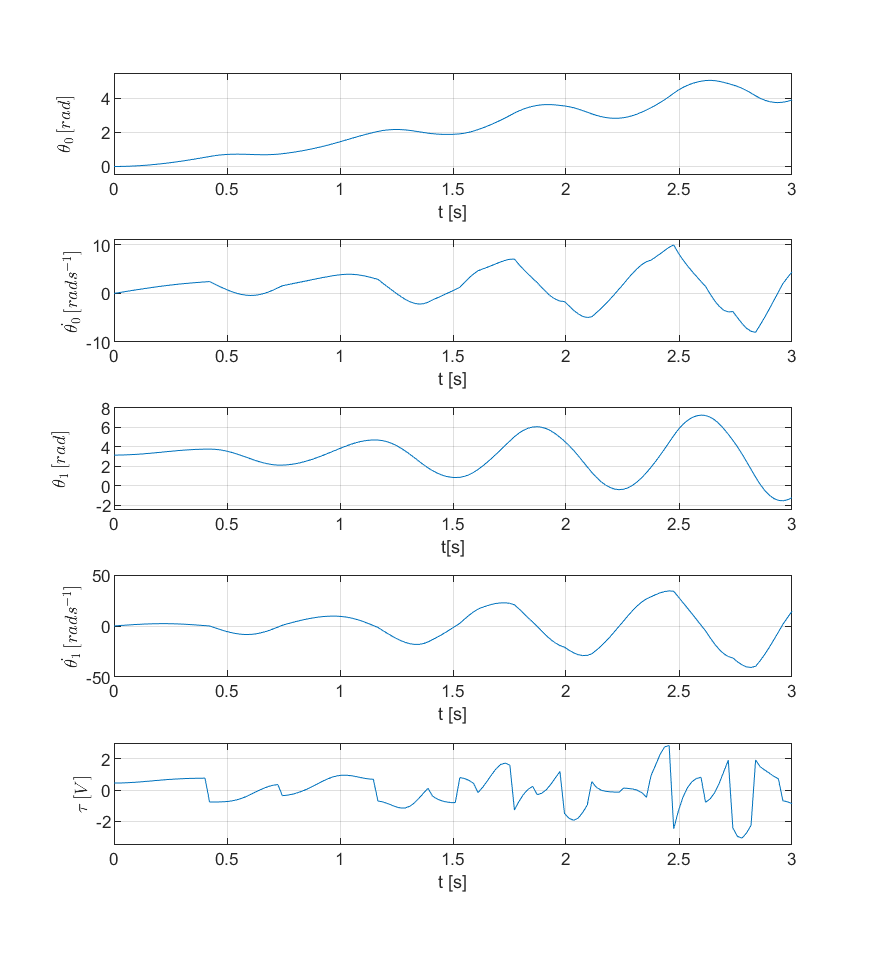
\includegraphics[width=1.1\linewidth]{images/Swing}
	\caption{Initial oscillation of the system by the Energy-Shaping controller. The plots depict, respectively, the individual states , the third of which is the controlled pendulum position $\theta_1(t)$, and the control input $\tau(t)$.}
	\label{swing}
\end{figure}
\newpage
\section{Heuristic Swing-Up Control}
To perform Swing-Up Control of the pendulum, a combined control strategy should be designed, because no MPC nor Swing-Up controller can not perform a Swing-Up control by itself. So the strategy of Heuristic Swing-Up Control is that at the beginning the pendulum is steady at the downside position and the Energy-Shaping controller is used to add the energy to the pendulum via its oscillation. As more energy is added to the pendulum, the greater the oscillations become. As the pendulum is close to the upright operation point, the control law switches from Energy-Shaping to MPC. And MPC finishes the Swing-Up Control by stabilizing the pendulum at the upright position.
\begin{figure}[H]
	\centering
	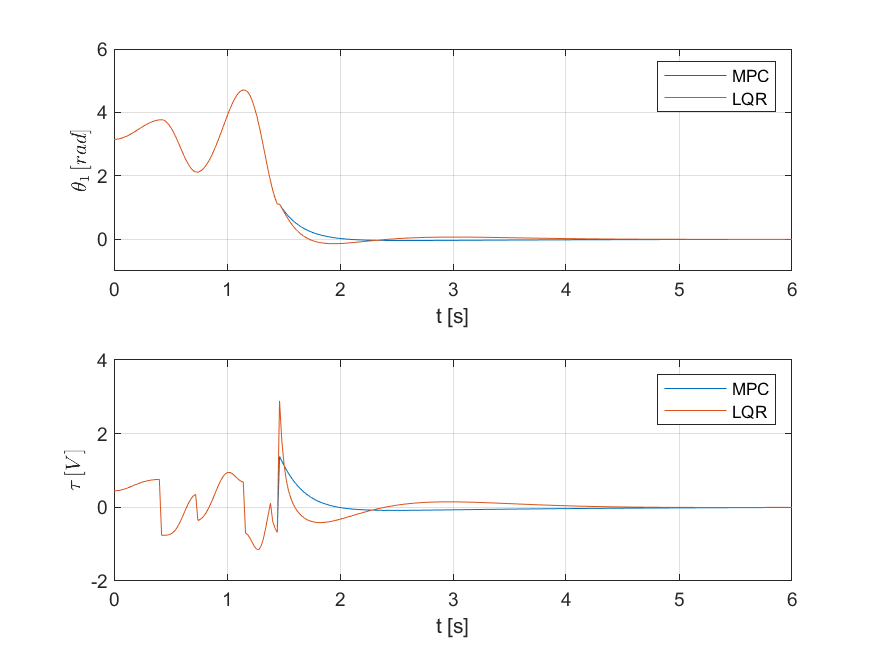
\includegraphics[width=1.1\linewidth]{images/MPC-LQR_Swing}
	\caption{Simulation result of the Swing-up control of the pendulum by Energy-Shaping+Mpc combined control strategy. The first plot depict the controlled pendulum position $\theta_1(t)$, and the second - control input $\tau(t)$.}
	\label{combo}
\end{figure}
\newpage
\section{Optimal Swing-Up Control}
The last control strategy is an Optimal Swing-Up Control. In this strategy, only one non-linear Model Predictive Controller (NMPC) is used to perform both the swing-up and the stabilization of the pendulum. Such control performance is possible due to the fact that in NMPC the non-linear model (\ref{nonlinmodel}) is used to predict the future evolution of the process.  Usage of this non-linear model, leads to a Non-linear Programing (NLP) problem, and solving a NLP problem is ot a trivial process. In this work a \textsc{MATMPC} toolbox is used \cite{MATMPC} to formulate and solve this problem.\\

 In general a NMPC problen can be formulated in similar form as linear MPC problem (\ref{mpc:linear}):
\begin{subequations}\label{nmpcgeneral}
	\begin{align}
	\min_{U}\ &\sum_{k=0}^{N-1} \lrp{\left\| \ui{Q}{x}x_{k}\right\|_2+\left\|\ui{Q}{u}u_{k}\right\|_2}\\
\text{s.t.}\ &x_{k+1} = f(x_{k}, u_{k})\qquad\qquad\qquad \ \   k \in \mathbb{N}_0^{N-1}\\
&x_0 = x(0)\\
&\ui{u}{min}\leq u_{k}\leq \ui{u}{max}\qquad\qquad\qquad\;   k \in \mathbb{N}_0^{N-1}
	\end{align}
\end{subequations}
The rules for weight matrices in NMPC strategy are similar to those, used in linear MPC strategy, except that to the arm is given more freedom and we are willing to invest more into control inputs. It's because of that the controller must not only stabilize the pendulum but also perform a swing-up.
\begin{equation}\label{NMPC:weights}
\ui{Q}{x} = \begin{bmatrix}
1&0&0&0\\
0&0.1&0&0\\
0&0&3&0\\
0&0&0&0.1
\end{bmatrix}, \quad \ui{Q}{u} = 0.1.
\end{equation}
Other NMPC parameters are shown in the following table
\begin{table}[H]
	\caption{NMPC parameters for the Optimal Swing-Up Control strategy}
	\begin{tabular}{l c c}
		\noalign{\hrule height 1pt}
		Parameter&Symbol&Value\\
		\noalign{\hrule height 1pt}
		Prediction horizon&$N$&$20$\\
		Initial condition&$x_0$&$\begin{bmatrix}0,0,\pi,0\end{bmatrix}^\intercal$\\
		Constraint on control input-upper bound&$\ui{u}{max}$&$\ \; \,10$\\
		Constraint on control input-lower bound&$\ui{u}{min}$&$-10$\\
		\hline
	\end{tabular}
\end{table}
The parameters are similar, that were used in MPC, except for the initial condition, that in case of NMPC the pendulum's steady downside position.\\

From a user perspective, the design of such an NMPC strategy, using \textsc{MATMPC} toolbox is trivial. You only have to set the NMPC parameters and define a prediction model (\ref{nonlinmodel}). And toolbox will automatically construct and solve the following NLP problem
\begin{subequations}\label{NLP}
	\begin{align}
	\min_{X,U}\ \frac{1}{2}&\sum_{k=0}^{N-1} (\left\| h_k(x_k, u_k)\right\|_2\ui{Q}{k}) + \frac{1}{2}\left\|h_N(x_N)\right\|_2\ui{Q}{N}\\
	\text{s.t.}\quad &x_{k+1} = \phi(x_{k},u_{k})\qquad\qquad\qquad\, k \in \mathbb{N}_0^{N-1}\\
	&x_0 = x(0)\\
	&\ui{u}{min}\leq u_{k}\leq \ui{u}{max}\qquad\qquad\qquad\;   k \in \mathbb{N}_0^{N-1}	
	\end{align}
\end{subequations}
where $h_k$ and $h_N$ are vector functions of state and control $(x, u)$, matrices $\ui{Q}{k}$ and $\ui{Q}{N}$ are the weights for each term for stage $k$. Matrix $\ui{Q}{k}$ have the size of $n_x+n_u\times N$ and matrix $\ui{Q}{N}$ have the size of $n_x\times 1$, where $n_x$ is a number of states and $n_u$ is the number of control inputs. Considering these rules and NMPC weight matrices (\ref{NMPC:weights}), the NLP matrices can be designed as
\begin{equation}\label{NLP:weights}
\ui{Q}{k} = \begin{bmatrix}
				1.0&\cdots&1.0\\
				0.1&\cdots&0.1\\
				3.0&\cdots&3.0\\
				0.1&\cdots&0.1\\
				0.1&\cdots&0.1
			\end{bmatrix}, \quad 
\ui{Q}{N} =	\begin{bmatrix}
				1.0\\
				0.1\\
				3.0\\
				0.1
			\end{bmatrix}.
\end{equation}
$\phi(x_{k},u_{k})$ is a numerical integration operator that solves the following initial value problem (IVP) and returns the solution at $t_{k+1}$.
\begin{equation}
0=\ui{f}{impl}\lrp{\dot{x}(t), x(t),u(t),t},\quad x(0)=x_k.
\end{equation}
In the next step, the listed above NLP problem is solved by the Sequential Quadratic Programming (SQP) method, which was described in the corresponding part of the thesis - Section \ref{SQP:theory}. Also, additional software must be installed:
\begin{itemize}
	\item \textbf{CasAdi} - to obtain the needed derivatives to perform optimization (\url{https://github.com/casadi/casadi/wiki}).
	\item \textbf{MinGW-w64 C/C++ Compiler} - to compile \textsc{MATMPC} modules into MEX functions with performance comparable to plain C/C++ solvers.
\end{itemize}
And with such setup, a Optimal Swing-Up control of the Pendulum can be performed
\newpage
\begin{figure}[H]
	\centering
	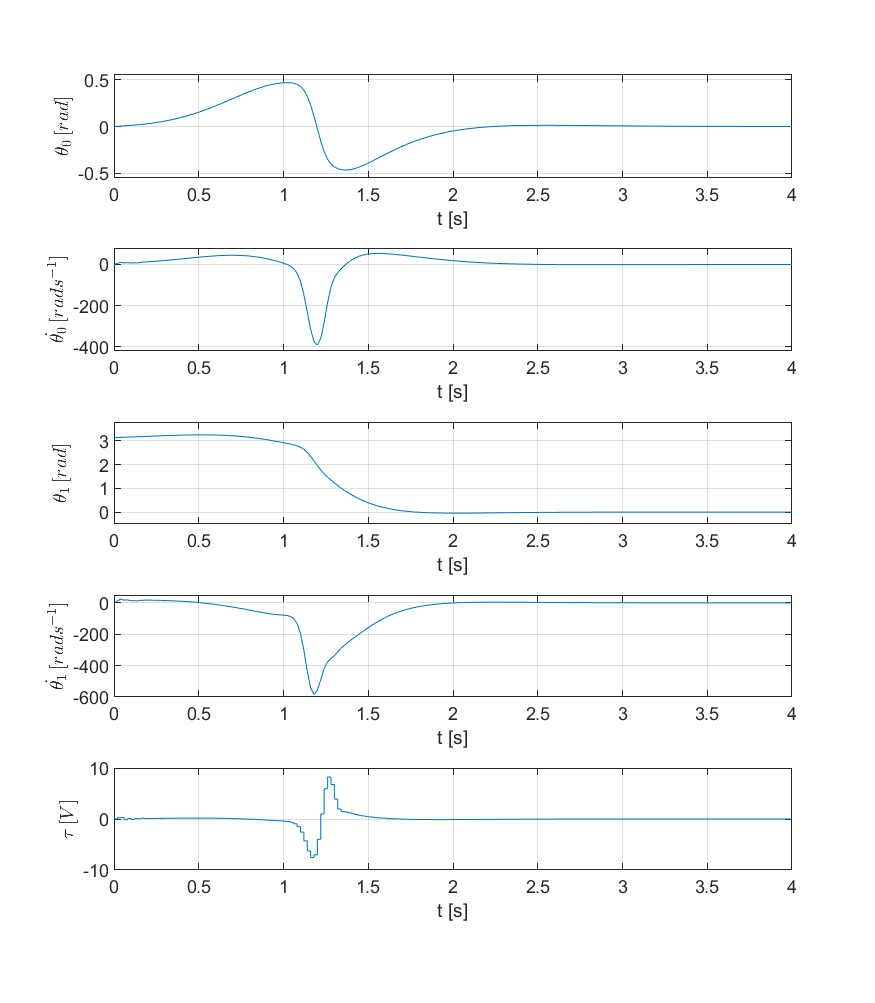
\includegraphics[width=1.1\linewidth]{images/NMPC}
	\caption{Simulation result of the Swing-up control of the pendulum by NMPC strategy.The plots depict, respectively, the individual states , the third of which is the controlled pendulum position $\theta_1(t)$, and the control input $\tau(t)$.}
	\label{NMPC:results}
\end{figure}
Considering the results in Fig.\ref{NMPC:results} we can conclude, that a non-linear predictive controller was designed correctly. It's capable to perform the Swing-Up control of the pendulum with its stabilization at the upright position without constraints violation. Also, the control was performed in an impressive time of $2.5\si{\second}$.
% conclusions
\chapter{Conclusions}
In this thesis, we have developed a control strategies to control a complex nonlinear oscillator what the Furuta pendulum is. The main task was to perform a Swing-Up control of the pendulum, with its stabilization at the upright position in an optimal way. But before we could proceed to the control strategies and control attempts, the mathematical dynamic model of the pendulum must be obtained first. For that purpose, a Lagrangian formulation of the system dynamics of the mechanical system was used. The Lagrangian formulation requires the construction of Lagrangian and Euler-Lagrange equations. As the Furuta pendulum has two degrees of freedom, two Euler-Lagrange equations were constructed. Then, by solving those equations, two equations of motion for both the Arm And the Pendulum were obtained. Further from those equations of motion, the nonlinear continuous-time State-Space dynamic model of the pendulum was derived. Then by linearizing that nonlinear model at the upright operation point, the linear dynamic model was acquired.

The next part of the thesis is a theoretical foundation for the individual controllers, used to control the pendulum. There are in total three controllers a Model Predictive Controller, an Energy-Shaping controller, and a Nonlinear Model Predictive Controller. For MPC was shown how to transform a problem of state regulation to the origin, to the standard Quadratic Programming problem. For Energy-Shaping controller was discussed the control law, which allows implementing such a state-feedback controller. For NMPC was shown how to solve a Nonlinear Programming problem by a numerical method, called Sequential Quadratic Programming.

The main task of the thesis is to perform Heuristic Swing-Up control and Optimal Swing-Up control of the pendulum. For Heuristic Swing-Up control an MPC and Energy-Shaping controllers were used. Initially, a Swing-Up controller is used to bring the pendulum in a range around the upright operating point, where the linear dynamic model is valid. Then the active controller switches to MPC, which further stabilizes the pendulum at the upright position. For the Optimal Swing-Up control the NMPC strategy was used. NMPC was designed through the \textsc{Matmpc} toolbox.

All controllers were designed and tested in \textsc{Matlab}. The obtained results are closer discussed in individual sections of the respective chapter.

% Appendices (Prílohy) comment by "%" if not neccesary
%\appendix
%\chapter{Resumé}
\label{ch:resume}

Resumé v slovenčine, sa píše v prípade, že záverečná práca ja napísaná v 
anglickom jazyku. Rozsah resumé tvorí 5-10\% rozsahu diplomovej práce.

%----------------------------------------------------------------%
%  The Backmatter !! Do NOT change the structure!!               %
%----------------------------------------------------------------%
% Bibliography to TOC
% do not remove
\backmatter
\providebibliography
\bibliography{bibfile}

%----------------------------------------------------------------%
%   The end of the document                                      %
%----------------------------------------------------------------%
\end{document}
